\documentclass[12pt,letterpaper]{article}
\usepackage{graphicx}
\usepackage{multirow}
\usepackage{authblk}
\usepackage{float}
\usepackage{rotating}
\usepackage{url}
\usepackage{lscape}
\usepackage{longtable}
\usepackage{subfigure}
\usepackage{natbib}
\usepackage{lineno}
\usepackage{amsmath,amsthm}
%\usepackage{fullpage}	
\usepackage{anysize}
\marginsize{1.0in}{1.0in}{1.0in}{1.0in}
\linespread{1.6}

\newcommand{\Pic}[2][0.85]{\begin{center}\includegraphics[width=0.8\textwidth,height=#1\textheight,keepaspectratio]{#2}
 \end{center} }


\title{Digital Elevation Models (DEMs) clustering for terrain modeling}
\author[1]{ E. R. Stefanescu }
\author[1]{A.K. Patra}
\author[2]{M. Bursik}
\affil[1]{Department of Mechanical and Aerospace Engineering, University at Buffalo, Buffalo, NY 14260}
\affil[2]{Department of Geology, University at Buffalo, Buffalo, NY 14260 }

\date{\today}


\begin{document}
\linenumbers
\maketitle

\begin{abstract}
We consider the problem of Digital Elevation Models (DEMs) segmentation 
in homogeneous regions, aiming for identification of plateaux, ridges, small drainages,
straight front slopes, valleys, and crests, in order to create ensembles of DEMs. These 
are then used in a systematic hazard analysis, resulting in a complete and complex
hazard maps. In the paper we explore and implement a method 
for segmentation using clustering, that is required / needed when we want to construct a 
sparse representation of the DEM.  The method -- spectral clustering, is extensively and 
successfully used in image segmentation. It is a complex 
method that accounts for the spatial correlation of the 
elevation points and has the advantage that it can be used for almost any application 
where relationships between topographic features and other components of landscapes 
are to be assessed. Here, the method is adapted for the case in 
which each data point has associated range of geomorphometric measures. 
\end{abstract}

\section{Introduction}
Information about topography is necessary for landscape evaluation, erosion studies,
hydrology and geophysical modeling, natural hazard prevention, etc. The classic way to 
incorporate relief units into a landscape assessment is to delineate them during field survey
or using stereo aerial photographs. This approach is relatively time-consuming and the results
depend on the subjective decision of the interpreter.
Several methods for the creation of landform elements using elevation-derived attributes are
described in the literature. Commonly, these techniques developed regions of homogeneity based
on common attributes and then classified those regions (or groups of regions) as elements. The 
most widely used techniques are: self organizing map \citep{Koh1995}, watershed segmentation 
\citep{Najman1996}, support vector machine \citep{Gunn1997}, segmentation using heuristic rules 
and fuzzy logic \citep{Sonka1999}, fuzzy $K$-means classification \citep{Burrough2000} and object-based 
image analysis \citep{Carleer2005}. Many of these techniques have drawbacks, especially when the
 method relies heavily on hydrological information and  requires data-specific knowledge; also these 
 methods don't incorporate autocorrelation between the same attribute at two locations in their models.
Digital Elevation Models (DEMs) are digital representations of terrain, and are represented as an 
array of squared cells (data points/ pixels) with an elevation associated to each data point. They can 
have different resolutions (5m, 30m, 90m, 120m, etc) and can be obtained from various methods 
(photometry, radar interferometry, laser altimetry, etc.). Usually the size of a DEM varies from
tens to hundreds of kilometers which can lead to thousands to millions of grid points. 
 
The aim of this paper is to quantify the variation in the output of a computational flow model for 
block and ash flows, when the model inputs, including the elevation values represented in the DEM, are
uncertain or given as a range of possible values. Integrating these variations in the possible flows 
as a function of input uncertainties provides well-defined data on the probability of hazard at
specific locations, i.e., a hazard map \citep{Keith}.  In particular, the focus here is on assessing the 
influence of DEM uncertainties and propose an improved method of generating ensembles of DEMs.

In this context, we would like to implement a more complex model segmentation of a DEM of Mammoth 
Mountain to create non-overlapping groupings of homogeneous regions. Mammoth Mountain (Fig.~\ref{fig:fig1}) 
is a volcano located in California and it was chosen due to the ease of obtaining data sets. 
\begin{figure}[ht!]
\center
      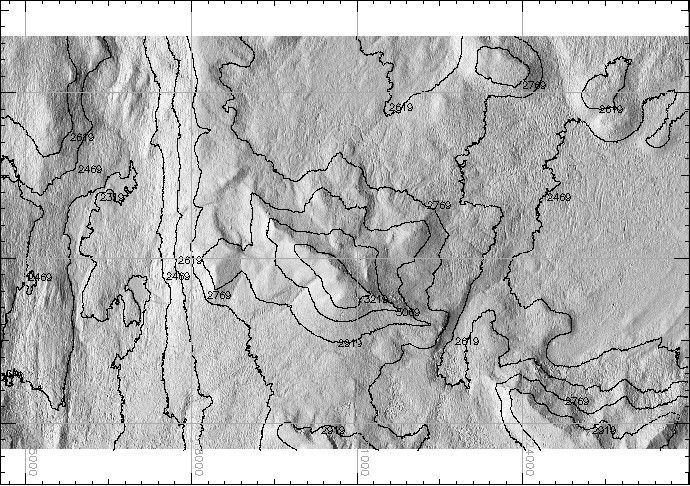
\includegraphics[width=10cm,height=11cm,keepaspectratio]{figs/Topsar5.png}\\
  \caption{Hillshade plot of the Mammoth Mountain  }\label{fig:fig1}
\end{figure}

\section{Methodology}
Segmentation is a broad term, covering a wide variety of problems and techniques. 
%Each segmentation method attempts to obtain a compact representation of its data set using some form of model of similarity.
Segmentation methods are based on some data point or region similarity
in relation to their local neighborhood. A variety of different methods have been proposed 
for image segmentation such as boundary-based segmentation, region-based segmentation and pixel-labeling. 
One view of segmentation is that we are trying to determine which components of the data set naturally 
``belong together". This is a problem known as \textit{clustering}. Clustering is difficult for a number of reasons. 
Real-life data may contain clusters of varying size and shape, whose number is unknown in advance. Noise 
and outliners can further complicate the task by connecting separate clusters. 
Spectral clustering was firstly developed in the context of graph partitioning problems \citep{Donath1973}, 
where the problem is to partition a weighted graph into disjoint pieces, minimizing the sum of the weights of the edges 
linking the disjoint pieces. In the graph the nodes represent the grid points and arcs represent affinities (``couplings") 
between nearby grid points. The final cluster assignments of the dataset can be achieved by optimizing some clustering 
criteria defined on the graph. The criteria of some spectral clustering methods are to optimize some cut value on an 
undirected graph, such as normalized cut \citep{ShiMalik2000}, ratio cut \citep{Hagen1992}, and min--max cut \citep{Ding2001}. 

To be able to perform the segmentation of the DEM in homogeneous regions
we need to specify a range of geomorphometric measures which can be extracted
from the surface. We define a \textit{feature matrix} of DEM attributes, consisting of elevation and 
first and second derivatives of elevation (slope, profile curvature and tangential curvature).
Slope and curvature are easily extracted from a DEM within a Geographical Information System (GIS).

In the next sections basic methodology for generating ensembles of DEMs using segmentation is presented, with emphasis 
on segmentation using spectral clustering.  Subsequent sections summarize the TITAN2D flow simulation tool and its use 
in a systematic hazard analysis. The hazard analysis tool itself uses ensembles of TITAN2D simulations to construct statistical surrogate models of flow outcomes at different locations as a function of model inputs, such as flow volume and pile initial 
location. Sampling of these surrogates leads to the construction of effective hazard maps that reflect the range of uncertainty 
in the model inputs.


\subsection{Spectral Clustering}
A digital representation of a terrain surface is an approximation of reality and is often subject to significant 
error. The error is usually not known in terms of both magnitude and spatial distribution. There are, in fact 
large uncertainties associated with the construction of DEMs. DEM vendors generally provide users with a
measure of vertical accuracy in the form of the root mean squared error (RMSE) statistic. One key feature of 
the DEM grid points, which are spatial data, is the autocorrelation of observations in space.  Generally, spatial 
autocorrelation refers to the correlation between the same attribute at two locations. Observations in close 
spatial proximity tend to be more related than observations at larger distances or separation. Based on this
assumption spectral clustering is performed to identify homogenous regions within a DEM. %\citep{Ng_Jordan, Luxburg}.

Compared with traditional clustering algorithms, spectral clustering has some advantages: can stably detect 
non-convex patterns and linearly non-separable clusters \citep{Sakai2009}, and can obtain the globally optimal 
solutions in a continuous domain by eigendecomposition  \citep{Archip2005}. As a discriminative approach, they 
do not make assumptions about the global structure of data. 
Instead, local evidence on how likely two data points belong to the same class is first collected and a global decision 
is then made to divide all data points into disjunct sets according to some criterion. Often, such a criterion can be
interpreted in an embedding framework, where the grouping relationships among data points are preserved as much
as possible in a lower-dimensional representation. What makes spectral methods appealing is that their global-optima 
in the relaxed continuous domain are obtained by eigendecomposition. However, to get a discrete solution from eigenvectors
often requires solving another clustering problem, albeit in a lower-dimensional space. That is, eigenvectors are treated as 
geometrical coordinates of a point set. Unfortunately, when the number of grid points (denoted as $n$) is large, spectral 
clustering encounters a quadratic resource bottleneck in computing pairwise similarity between $n$ nodes and storing 
that large matrix. Moreover, the algorithm requires considerable computational time to find the smallest $k$ eigenvalues of 
a Laplacian matrix. Eigenvalues and eigenvectors are at the heart of spectral clustering algorithms, and in spite of their 
importance, existing eigensolvers do not scale well. Fast computation schemes for spectral clustering have been proposed 
by  different authors. They focus on the eigenvector computation of a graph Laplacian defined by a matrix of data similarities.
The Krylov subspace methods \citep{Mahadevan2008}, are iterative algorithms for finding leading eigencomponents of a sparse 
matrix, while \cite{Dhillon2007} assume the availability of the similarity matrix and propose a method that does not use eigenvectors.
\cite{Fowlkes2004} propose using the Nystr\"{o}m approximation to avoid calculating the whole similarity matrix. In this paper we are 
using a method proposed by \cite{Song2008}, which parallelize spectral clustering on distributed computers to address
resource bottlenecks of both memory use and computation time.

\subsubsection{Approach}
For a given data set $P = \{ p_1,\dots, p_n \in R^d \}$, spectral clustering finds a set of data clusters, $\{C_1,\dots, C_k \subset P\}$,
on the basis of spectral analysis of a similarity graph. Spectral clustering builds a weighted graph $G(V,E)$, where $V$ represents vertices and $E$, edges. 
We represent each elevation point as a node in the graph $G$ and the links between the adjacent data points will form the edges of the graph. Spectral clustering partitions data points into groups such that the members of a group are similar to each other and dissimilar to data points outside of the group. Given data points, an affinity matrix can be represented by a weighted adjacency matrix $W \in \mathcal{R}^{n\times n}$, where $w_{ij}$ is a measure
of the similarity between grid point $i$ and grid point $j$. The affinity matrix is used to preserve the local structure of the patterns. It expresses the degree of similarity between points, and
it must have the following properties: i) non-negative; ii) symmetric; iii) invertible.
We have chosen the heat kernel for calculating the affinity matrix, as:
%\begin{align}
%W_{i,j} = \exp ( -  \frac{\lVert x_i - x_j \rVert^2}{\sigma^2} )
\begin{equation}
{\mathbf W_{ij}} = \left\{
\begin{array}{rl}
\exp{\frac{- \parallel F(i) - F(j) \parallel}{\sigma_F^2}}*exp{\frac{- \parallel x(i) - x(j) \parallel}{\sigma_x^2}}, & if \parallel x(i) - x(j) \parallel \le r\\
0, & \qquad \text{otherwise},
\end{array} 
\right.
\label{eq:eq1}
\end{equation} 
where $F(i)$ represents the DEM feature vector for node $i$, and $x(i)$ represents the coordinate location of $i^{th}$ node.
$\sigma_F $ and $\sigma_x$ are positive tuning parameter that controls the decay of the affinity \citep{Tung2010}.
The graph partitioning can be interpreted as a minimization problem of an objective function. Common objective functions are
the ratio cut (Rcut), normalized cut (Ncut) and min--max cut (Mcut) expressed as:
\begin{align}
Rcut (C_1,\dots,C_k) = \sum_{l=1}^k \frac{(C_l, P \setminus C_l)}{card\; C_l} 
\label{eq2}
\end{align}
\begin{align}
Ncut C_1,\dots,C_k) = \sum_{l=1}^k \frac{(C_l, P \setminus C_l)}{cut (C_l, P)}
\label{eq3}
\end{align}
and
\begin{align}
Mcut (C_1,\dots,C_k) = \sum_{l=1}^k \frac{(C_l, P \setminus C_l)}{cut (C_l,C_l)} 
\label{eq4}
\end{align}
Here, $cut(X,Y)$ is the sum of the edge weights between $\forall p \in X$ and $\forall p \in Y$, $P\setminus C_l$ is the complement
of $C_l \subset P$, and $card\; C_l$ denotes the number of points in $C_l$.
The degree $d_i$ of node $i$ is the sum of all edge weights incident on $x_i$:
\begin{align}
d_i = \sum_{j=1}^n w_{ij}
\end{align} 
The \textit{degree matrix D $\in \mathcal{R}^{n \times n}$} is defined as the diagonal matrix with the degrees $d_1, \dots, d_n$ on the diagonal, while the %normalized
unnormalized graph Laplacian matrix $L \in \mathcal{R}^{n \times n}$ is defined as \citep{Chung1997}:
\begin{align}
%L = I - D^{-1/2}WD^{-1/2}
L = D - W
\end{align}
Let $h_l$ be an $n-$dimensional vector indicating the members of the cluster $C_l$ by its binary components. The minimization 
problem of any objective function in Eqs. \ref{eq2}, \ref{eq3} and \ref{eq4} can be rewritten as a trace minimization problem under a 
constraint on a matrix $H = [h_1 \dots h_k]$:
\begin{align}
\min_H tr (H^\top L H) \; subject \;to\;  H^\top L H = I.
\label{eq5}
\end{align}
The matrix $N$ is equal to $I, D$ or $W$ for Rcut, Ncut or Mcut, respectively \citep{ShiMalik2000, Ng2002}. The spectral clustering algorithms were derived from the
minimization problem in Eq. \ref{eq5} by relaxing the binary constraint on $h_l$. The relaxed trace minimization for $H \in \mathcal{R}^{n \times k}$ is the generalized eigenvalue problem \citep{vonLuxburg2007}:
\begin{align}
LH =NH\Lambda
\label{eq6}
\end{align}
The eigenvectors for Ncut and Mcut are identical due to this relaxation, while for Ncut, Eq.\ref{eq6} can be converted into
a normal eigenvalue problem:
\begin{align}
SZ = Z\Delta
\end{align}
where
\begin{align}
S = S_{sym} =  D^{-1/2}WD^{-1/2}, \; Z = D^{1/2} H \; and \; \Delta = I - \Lambda
\end{align}
or
\begin{align}
S=S_{rw} = D^{-1} W, \; Z = H \; and \; \Delta = - \Lambda
\end{align}
The above method leads to the normalized graph Laplacians defined as:
\begin{align}
L_{sym} = I - D^{-1/2}WD^{-1/2} \; and \; L_{rw} = I - D^{-1} W
\end{align}
$L_{sum}$ is a symmetric matrix, while $L_{rw}$ it is closely related to a random walk. A more detailed 
description for normalized graph Laplacian can be found in \citet{Chung1997}.
The data clustering by graph-cut boils down to the eigenvalue decomposition problem of $S$ for finding 
the cluster indicators $h_1, \dots h_k$. %The solution is the matrix of the first $k$ eigenvectors of $S$.
% followed by a K-means cluster in
%the eigenvector space. 
%$L$ satisfies the following properties:
%\begin{itemize}
%\item For every $f \in \mathcal{R}^n$ we have :
%\begin{equation}
%f' L f = \frac{1}{2} \sum_{i,j=1}^n w_{ij}(f_i - f_j)^2.
%\end{equation}
%\item $L$ is symmetric and positive semi-definite.
%\item The smallest eigenvalue of $L$ is $0$ and the corresponding eigenvector is the constant unity vector $1$.
%\item $L$ has $n$ non-negative, real-valued eigenvalues $0=\lambda_1 \le \lambda_2 \le \cdots \le \lambda_n$.
%\end{itemize}
%The most interesting aspect of spectral clustering is the mapping of the data points into a new space with
%$k$-dimensions by means of eigenvector decomposition. 
These eigenvectors induce an embedding of the data points in a low-dimensional subspace wherein a
partitioning based on the normalized cut (NCut) can be used. The solution of the minimization problem can be 
obtained from the Fiedler eigenvector \citep{Stella2003}.
 The steps involved in DEM segmentation using spectral clustering are summarized in Figure ~\ref{fig:fig2}.
\begin{figure}[ht!]
\center
      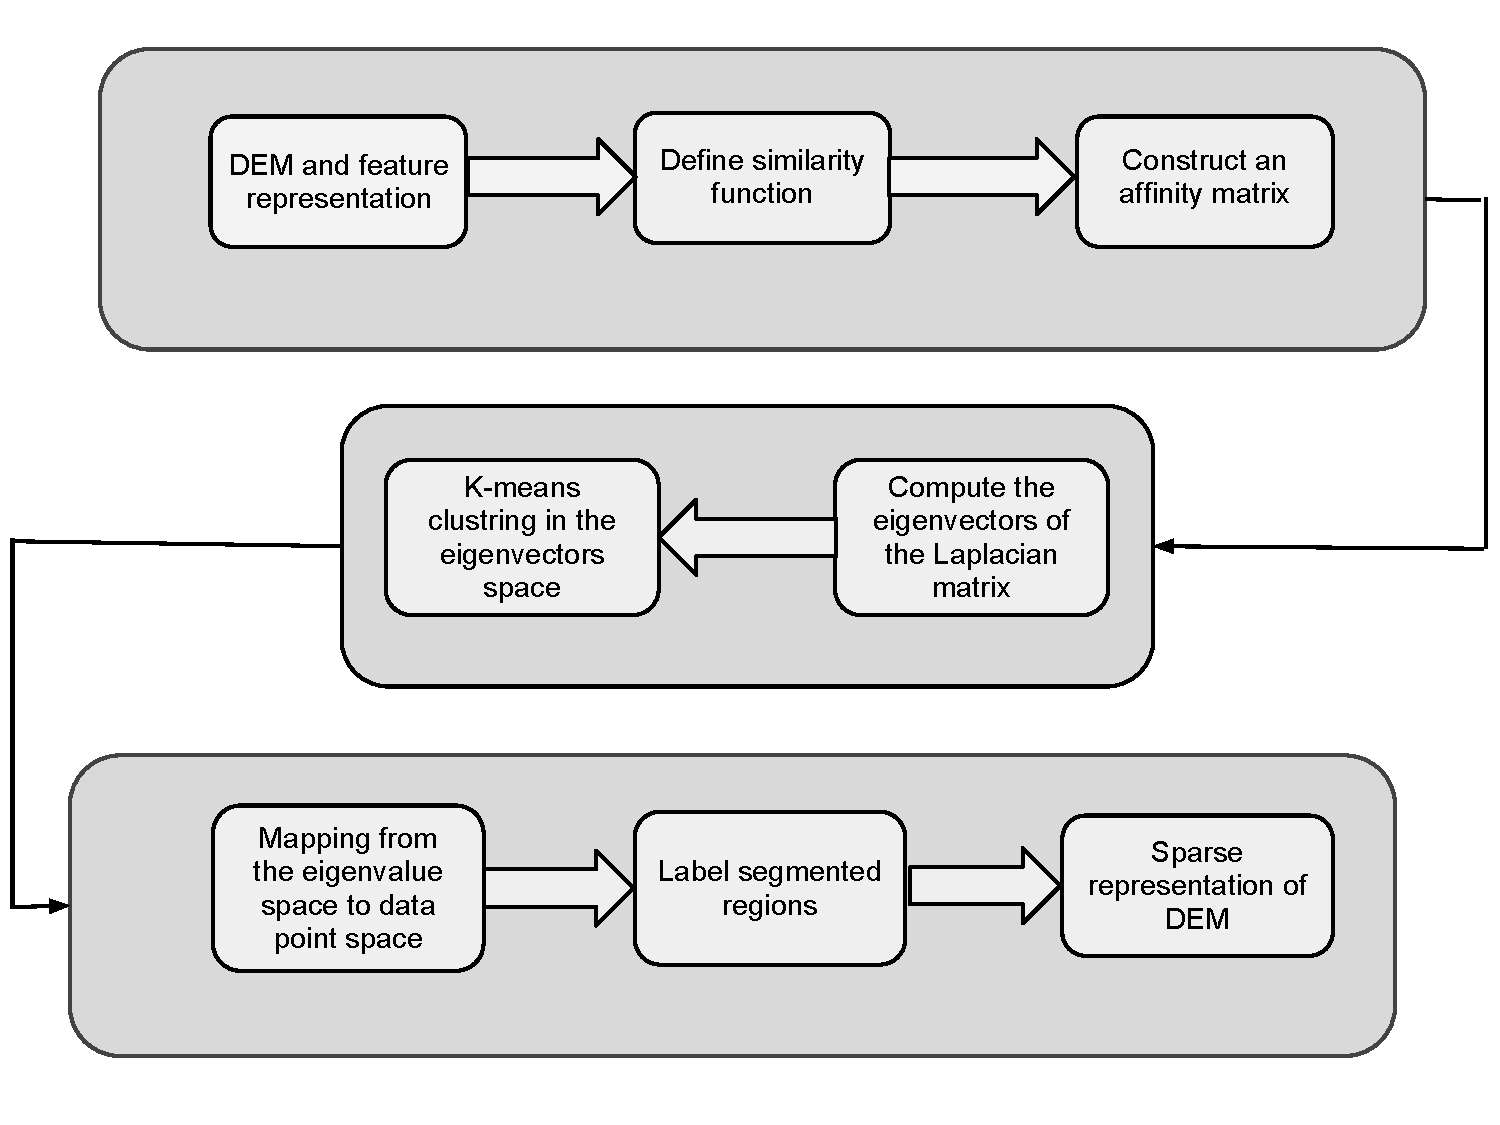
\includegraphics[width=10cm,height=11cm,keepaspectratio]{figs/Spectral_flow.pdf}\\
  \caption{Spectral clustering for DEM segmentation workflow}\label{fig:fig2}
\end{figure}
 
%In Figure~\ref{fig:fig3} the Spectral Clustering was performed for $\sigma=1$ and a DEM of 120m resolution. 
%\begin{figure}[ht!]
%\center
%      \includegraphics[width=10cm,height=11cm,keepaspectratio]{Spectral1.pdf}\\
%  \caption{Spectral Clustering $\sigma =1 $  }\label{fig:fig3}
%\end{figure}
%\begin{figure}[ht!]
%  \begin{minipage}[b]{0.5\textwidth}
%    \begin{tabular}{c}
%      \includegraphics[width=7cm,height=8cm,keepaspectratio]{pics/T5_K4.pdf}\\
%      (a)
%    \end{tabular}
%  \end{minipage}
%  % \hfill
%  \begin{minipage}{0.5\textwidth}
%    \begin{tabular}{c}
%      \includegraphics[width=7cm,height=8cm,keepaspectratio]{pics/T5_K6.pdf}\\
%      (b)
%    \end{tabular}
%  \end{minipage}
%  \caption{a) Hillshade plot of the Mammoth Mountain b) 3D plot Mammoth Mountain }\label{fig:fig1}
%end{figure}
%As a next step in our project we will try to improve the way the affinity matrix is define in spectral clustering,
%such that both location and the feature matrix to be incorporated. Also, a Gaussian Mixture clustering will be
%implemented.

\subsubsection{Parallel implementation}
When the number of data points (n) is large, the computational complexity of spectral decompositions can reach $O(n^3)$ ($W$ dense). If the affinity matrix $W$ is define as in Equation ~\ref{eq:eq1} then its construction takes $\mathcal{O}(n^2d)$ flops, which 
can be also computationally intensive if the data cardinality $n$ or dimensionality $d$ is large.
\cite{Chen2011} investigate approaches for large-scale spectral clustering and propose a parallel implementation, which is also
adopted in this paper. The strategy to address the computational and memory difficulties involves distributing $n$ data instances 
onto $p$ distributed machine node. On each node, parallel spectral clustering (PSC) computes the similarities between local data and the whole set in a way that uses minimal disk I/O. Then PSC stores the eigenvector matrix on distributed nodes to reduce 
per-node memory use. Together with parallel eigensolver and $K$-means, PSC archives good speedup with large data sets.

%\subsubsection{$K$-means}
%Since $EM$ algorithm convergences to local maxima, initialization is very important. The initialization 
%of the Gaussian mixture parameters is done using $K$-means.
%$K$-means is essentially a sorting and binning procedure where the user determines the number 
%of bins / clusters to be used and the rules for sorting. The
%$K$-means procedure sorts a set of data points into a specified number of clusters based on the 
%feature vector for each data point [3].
%Comparison of the $K$-means algorithm with the $EM$ algorithm for Gaussian mixtures shows that they are
%very similar [6]. The $K$-means algorithm uniquely assigns each data point within a cluster whereas the$EM$ algorithm makes
%the assignment based on the posterior probabilities.
%The data set available is a 5m DEM, covering an area of $\approx 94 km^2$ which results in $\approx 3$ millions 
%data points. To speed up the computational time, the majority of the analysis was performed on a decimated 
%DEM having a 120m resolution and 6550 data points. 
%The following steps are implemented for the $K$-means algorithm:
%\begin{itemize}
%\item We choose $k$ = 4, 6 and 10 clusters from the DEM. There are $\mu_1, \mu_2, \cdots , \mu_k$ means 
%that we use for initialization.
%\item For each elevation point the nearest mean is calculated.
%\begin{align}
%c_{i} = \underset{\mu_j \in \{\mu_1, \mu_1, \cdots, \mu_k \}}{\operatorname{argmax}} (x_i - \mu_j)^2
%\end{align}
%\item The means values were updated based on the elevation points assigned to them. 
%\item The above steps were repeated until the locations of the means were no longer changing
%by a significant amount.
%\end{itemize}

\section{DEM ensembles}
When propagating uncertainty in DEMs through a geophysical system, stochastic methods are considered to 
be an effective way to estimate the probability density function of outputs by addressing uncertainties present in 
initial conditions and in model approximations.
In previous work \cite{stefanescuPRS2012} presented a basic methodology for generating
ensembles of DEMs representative of the true DEM. Here, we are extended the methodology at the cluster level, 
by making the assumption that each homogenous regions has its own error model which leads to different random 
fields. The random fields are used in creating multiple equally likely representations of an actual terrain
surface, following the approached suggested by \cite{Ehlschlaeger_1994}.
A normal distribution (mean of 0.0 and variance of 1.0) of maps or realizations is computed to reproduce the 
spatial autocorrelation encountered in the original error surface, filtered using a Gaussian convolution filter, with 
kernel sizes derived from autocorrelation analysis of the original error surfaces.
The random field function derives its spatial dependence from the use of a distance
based decay filter function. The following equation is used to
generate the random field:
\begin{align}
  &Z(\mathcal{U})= \frac{\sum_v w_{u,v}\epsilon_v}{\sqrt{\sum_v
      w_{u,v}^2}}, \quad u\in \mathcal{U}, \; v \in \mathcal{V}
 \label{eqn1}
 \end{align}
 \begin{align}
   w_{u,v} = \left\{ \begin{array}{ll} 1 & \quad :d_{u,v} \le F \\
       \left(1- \frac{d_{u,v} - F}{D - F} \right)^E & \quad F <
       d_{u,v} \le D, \; u \in \mathcal{U}, \; v \in \mathcal{V}\\ 0 &
       \quad :d_{u,v} > D
\end{array} \right.
\label{eqn2}                                                    
\end{align}
where $\mathcal{V}$ is the set of points potentially influencing
points in a given area, $\mathcal{U}$, $w_{u,v}$ is the spatial
autocorrelative effect between points $u \in \mathcal{U}$ and $v \in
\mathcal{V}$, $\epsilon_v$ is a Gaussian random variable with a mean of 0 and
variance of 1, $d_{u,v}$ is the distance between $u$ and $v$, $D$ is
the minimum distance of spatial independence, $E$ is the distance
decay exponent, and $F$ the distance at which errors are completely
correlated.

A set of random fields are created for each homogenous region/ cluster and are calibrated to 
the spatial variation of the field being simulated using a correlogram function. This is done by
fitting the correlogram and choosing the best descriptive parameters
of the random field (the minimum distance of spatial independence, the
correlated distance decay exponent and the filter parameter) in a
weighted least-square estimator.  After running hundreds of tests with
multiple combinations of $D$, $E$ and $F$, the best random field was 
found by fitting the error map characteristics such that the sum of
least squares difference between an error field's correlogram and the
target correlogram is minimized.

Each error realization was added
to the ``true'' DEM indicated as $m(\mathcal{U})$, to generate equally probable realizations of the
topography for the error structure of a DEM under consideration:
\begin{equation}
 R(\mathcal{U})=m(\mathcal{U})+m(m(\mathcal{T}))+(m(s^2(\mathcal{T}))\cdot \epsilon)\cdot Z(\mathcal{U})
\label{eq:one}
\end{equation} 
where $R(\mathcal{U})$ is a realization of the elevation dataset $m(\mathcal{U})$, $\mathcal{T}$ is a
group of sets of spatially uncorrelated sample points in $m(\mathcal{U})$, and $\epsilon$
is a Gaussian random variable with mean 0.0 and variance 1.0. $m(m(\mathcal{T}))$ and
variance $m(s^2(\mathcal{T})$ is mean and variance, respectively, of all sets in 
$\mathcal{T}$. $Z(\mathcal{U})$ specifies the random field as
defined in Equation ~\ref{eqn1} for each homogenous region. 

 \begin{figure}[H]\centering
\subfigure[]{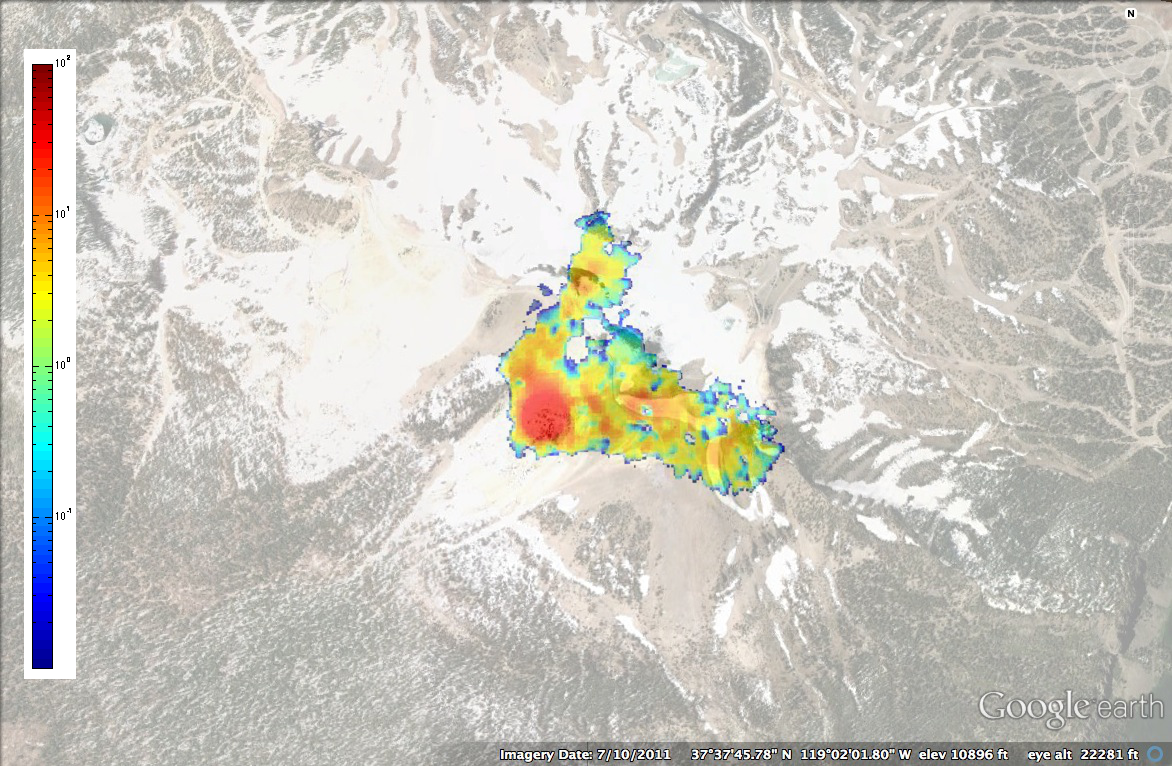
\includegraphics[width=3in]{figs/Flow_map_179_noclust_legend.png}}
\subfigure[]{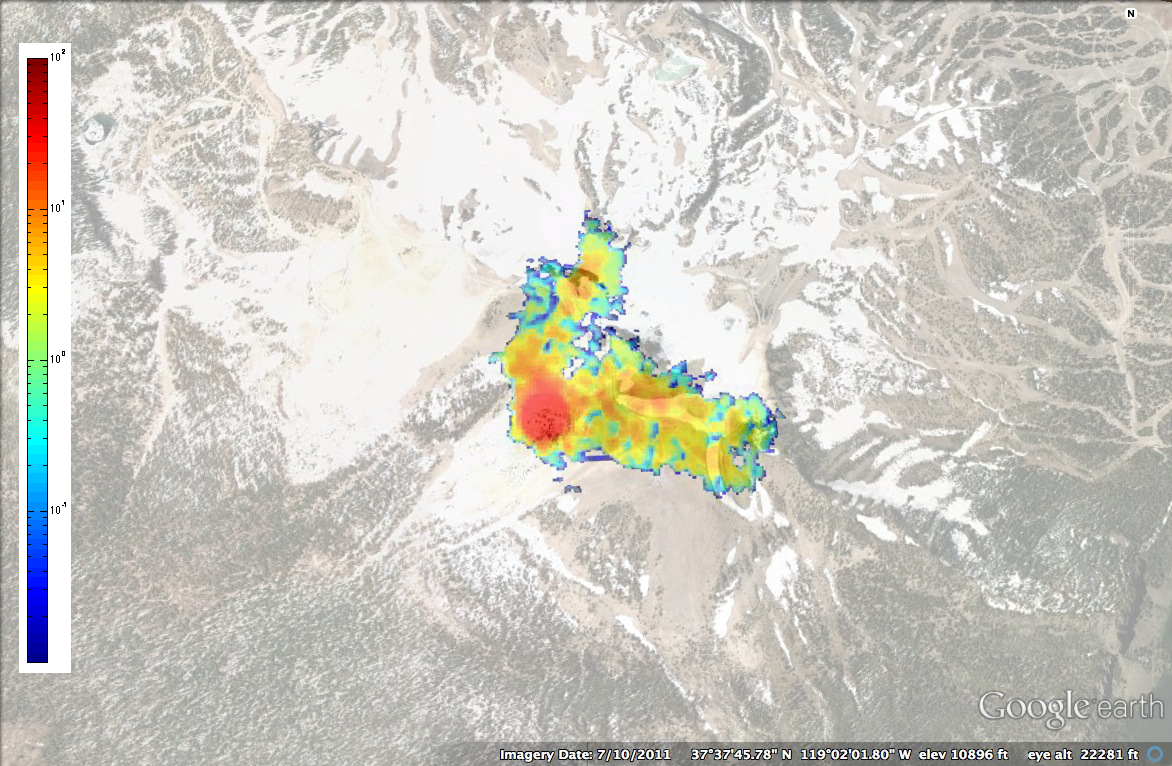
\includegraphics[width=3in]{figs/Flow_map_179_clust_legend.png}}
\subfigure[]{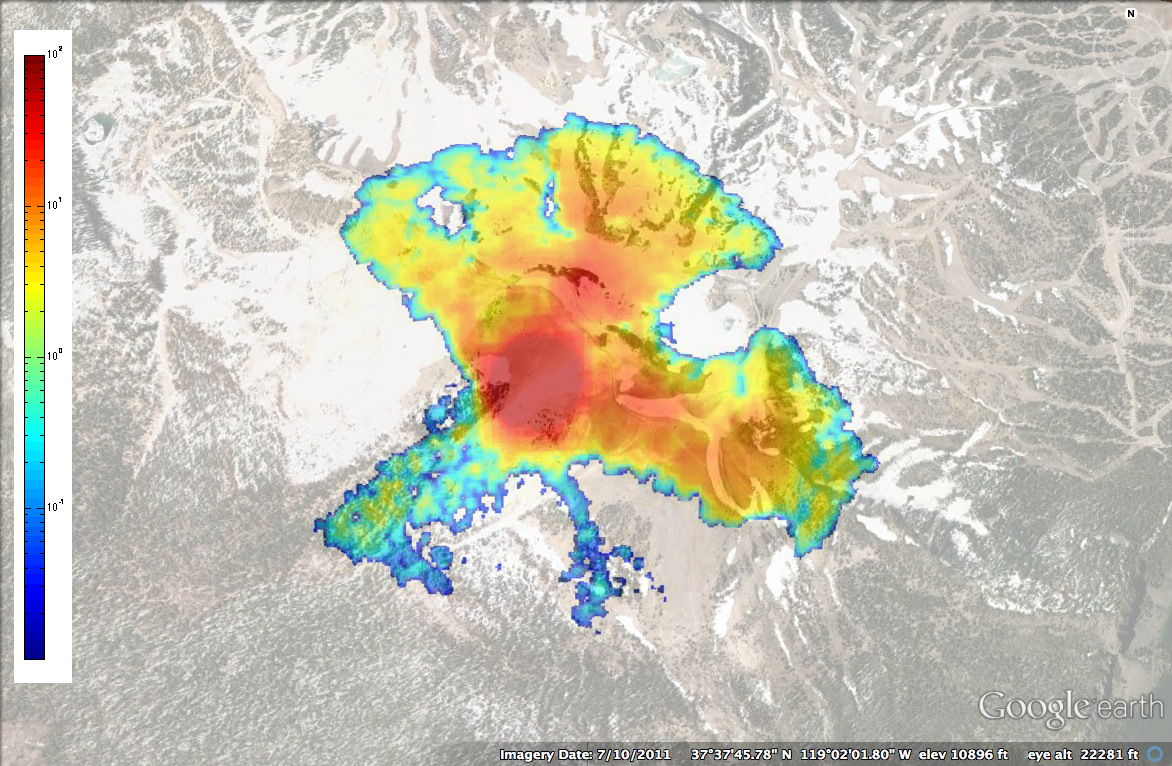
\includegraphics[width=3in]{figs/Flow_map_523_noclust_legend.png}}
\subfigure[]{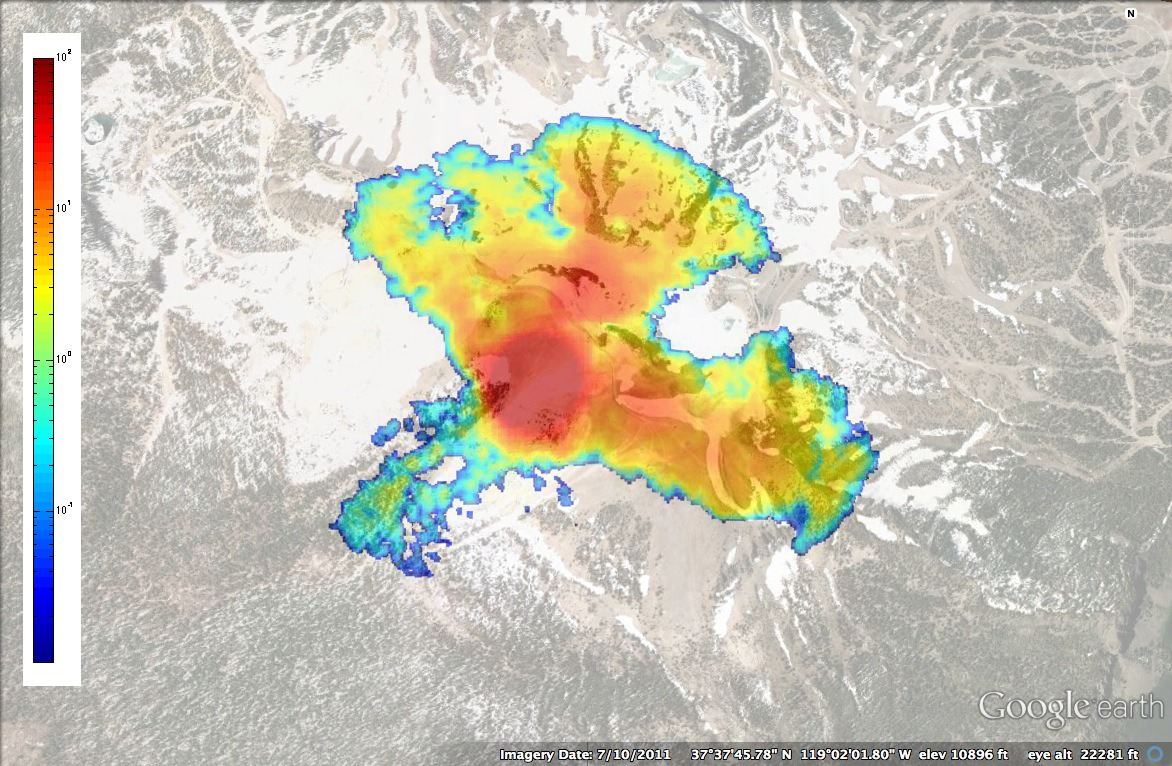
\includegraphics[width=3in]{figs/Flow_map_523_clust_legend.png}}
\caption{Flow maps for two selected parameters values when DEM was created using a) no cluster b) cluster  }
\label{fig:rapido}
\end{figure} 

\section{Flow simulator}
The threat of avalanches, block-and-ash flows, and mud-flows at volcanoes is a major global problem.
These are complex phenomena and involve physics at multiple spatial and temporal scales. Developing satisfactory models and computational simulations of potential debris flows on natural terrains and integrating them with appropriate geographical information is difficult but extremely necessary. In recent years, many significant advances have been made in the modeling and simulation of such flows by taking advantage of new models of the physics, new stable and accurate solution schemes for nonlinear hyperbolic systems, and the wide availability of high-performance computers.

Hazard maps are one of the most important instruments \citep{Sheridan2010} for representing areas of potential inundation by
dangerous phenomena at volcanoes. One major problem with using model to construct hazard maps is the strong dependence on the outcome on the choice of model parameters, such as bed friction, initial volumes and terrain. 

\subsection{TITAN2D}
TITAN2D \citep{Patra2005, sheridan_2005} was developed for modeling dry geophysical granular flows,
such as debris avalanches and block and ash flows. The TITAN2D code
combines numerical simulations of a natural granular flow with digital
terrain data. It is based on a depth-averaged model for an
incompressible granular materia governed by Coulomb-type friction
interactions \citep{Savage1989}.  The governing equations are obtained
by applying conservation laws to the incompressible continuum,
providing appropriate constitutive modeling assumptions, and then
taking advantage of the shallowness of the flows (flows are much
longer and wider than they are deep) to obtain simpler depth-averaged
representations \citep{BuPaPi05}. The motion of the material is
considered to be gravitationally driven and resisted by both internal
and bed friction. The stress boundary conditions are: no stress at the
upper free-surface and a Coulomb-like friction law imposed at the
interface between the material and the basal surface.

A principal feature of TITAN2D is the incorporation of topographical data from geographic 
information system (GIS) sources into the simulation and grid structure. Topographic data 
are included in the simulation through a preprocessing routine in which the digital
elevation data are imported. TITAN2D performs flow simulations on a DEM of a desired 
region, the simulation accuracy being highly dependent on the level of the DEM resolution 
and quality \citep{stefanescu1}. 

Inputs to the code are the size and location of the initial volume,
the internal and bed friction and the DEM. \citet{Keith} presented
several methods for characterizing the effect of input data
uncertainty on model output -- except DEM, where uncertainty associated 
with spatial parameters like terrain elevation were not well understood.
The output -- the flow height at every grid point
at every timestep -- is a complete description of the mass flow over realistic terrain.

%The stochastic input is defined as 
We define the stochastic input as $\Omega = (UTM_E, UTM_N, \textbf{V}, \theta_r)^\top$. 
$UTM_E$ and $UTM_N$ are the East and North, respectively coordinates ( UTM values )
of the location of possible vents. These are considered to be uniform distributed around 
321095 E and 4166433 N, within 400m radius. \textbf{V} is the initial volume of material,
uniform distributed between $10^{5}$ $m^3$ and $10^{7.5}$ $m^3$. $\theta_r$ includes the DEM uncertainty as described 
in Section 3. We ran 1024 flow simulations at design points in the region of the input space. These 1024
design points were chosen according to a Latin hypercube design, which is a space-filling 
design. This has been proven very successful for all-purpose designs of computer experiment runs
since they require relative few design points per input to ``fill" the design space \citep{Sacks1989}. 
%
%\subsection{Bayes Linear Model}
%There are numerous ways to create a volcanic hazard map based on
%computational fluid dynamics modeling. One way to approximate the hazard  map is to use Monte Carlo
%simulations for selected flow model, given a large number of samples of input parameters, defined
%over the uncertain domain $\Omega$. It is well known that running Monte Carlo simulations involves humongous 
%computational effort for reasonably large number of samples. Another approach is Polynomial Chaos (PC) framework, 
%which can be applied to quantify the effect of uncertainty involved in input parameters on a forward model outcome 
%\citep{ICCS2013}. 
%Here the Bayes Linear method (BLM) \citep{blm1tutor} was used to construct an
%emulator. An emulator is a regression surface based on a
%representative sample of simulations at selected inputs, accompanied
%by statistical error bounds. Equipped with this surface, output values
%at new (untested) input values need not be run.  Instead output
%results can be determined by evaluating the emulator. Given prior beliefs $(B)$ of mean and variance, the BLM
%updates these beliefs conditioned on the data $(D)$.  Note that
%``data'' generally here refers to the output of computationally
%expensive physics based simulators.  Because only the first two
%moments of a distribution are determined, the BLM is exact only for
%Gaussian distributions. Given the prior expectation $E[B]$ and variance
%$var(B)$, the BLM updates are
%\begin{eqnarray} \label{blupdate}
%E_D(B) &=& E[B] + cov(B,D) (var(D))^{-1} [D-E[D]] \\ \nonumber
%var_D(B) &=& var(B) - cov(B,D) (var(D))^{-1} cov(D,B)
%\end{eqnarray}
%These update formulae can be derived by minimizing the mean square
%error $(B - a^T D)^2$ between $B$ and some linear combination of the
%data. Thus the BLM update can be viewed as the projection of the set
%of prior beliefs onto the span of the data. A more detailed description of the method
%can be found in \cite{dalbeythesis}.

\section{Results}

The data set available is a 5m DEM, covering an area of $\approx 94 km^2$ which results in $\approx 3$ millions 
data points. To speed up the computational time, the majority of the analysis was performed on a decimated 
DEM having a 120m resolution and 6550 data points. 

\begin{figure}[H]
  \begin{minipage}[b]{0.5\textwidth}
    \begin{tabular}{c}
      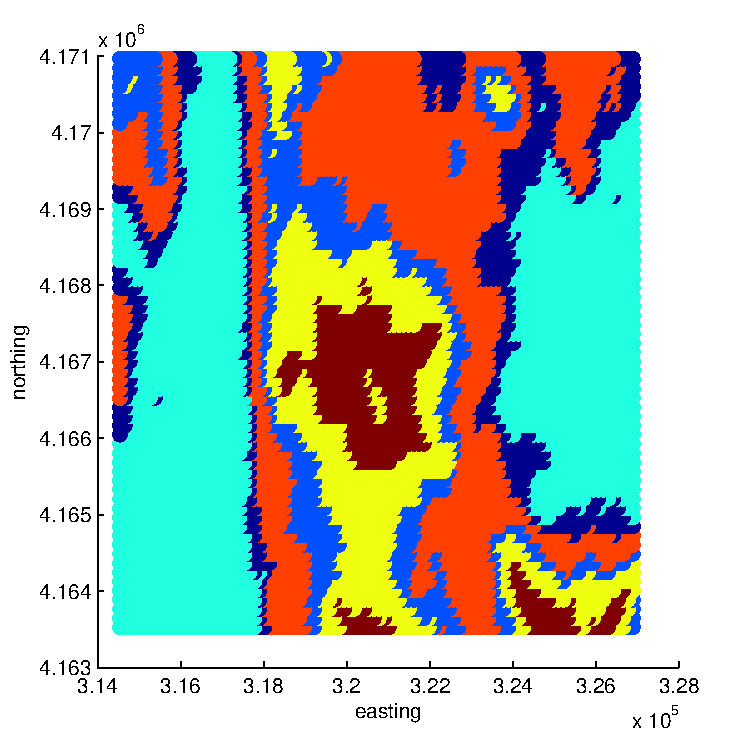
\includegraphics[width=8cm,height=7cm,keepaspectratio]{figs/Spectral1_old.pdf}\\
      (a)
    \end{tabular}
  \end{minipage}
  % \hfill
  \begin{minipage}{0.5\textwidth}
    \begin{tabular}{c}
      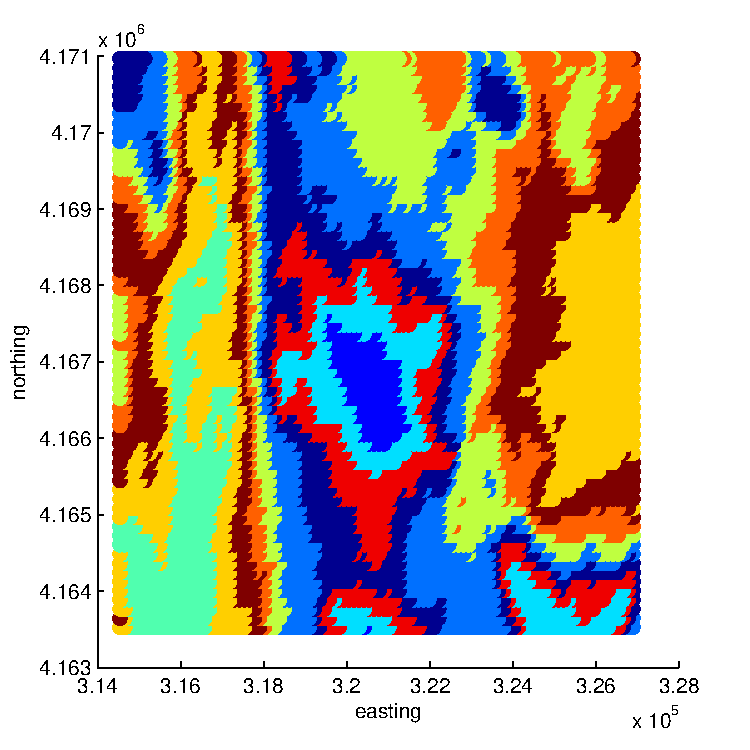
\includegraphics[width=8cm,height=7cm,keepaspectratio]{figs/T30_K10.pdf}\\
      (b)
    \end{tabular}
  \end{minipage}
  \begin{minipage}[b]{0.5\textwidth}
    \begin{tabular}{c}
      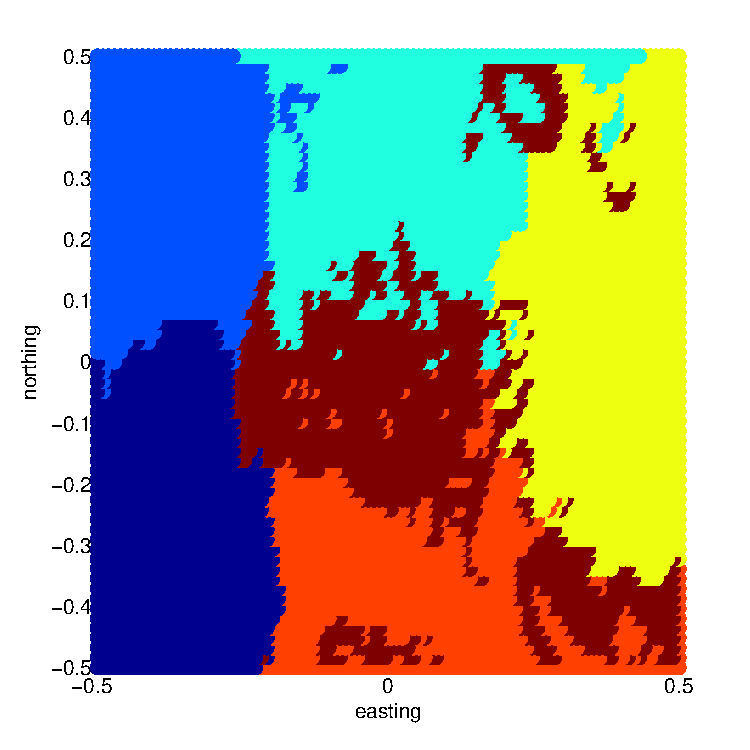
\includegraphics[width=8cm,height=7cm,keepaspectratio]{figs/Spectral2.pdf}\\
      (c)
    \end{tabular}
  \end{minipage}
  % \hfill
  \begin{minipage}{0.5\textwidth}
    \begin{tabular}{c}
      \includegraphics[width=8cm,height=7cm,keepaspectratio]{figs/Spectral1.pdf}\\
      (d)
    \end{tabular}
  \end{minipage}
   \caption{Spectral Clustering for a) K=6 -- one feature b) K=20 -- one feature c) K=6  where $\sigma_F = 0.8$ and $\sigma_x = 1$ -- 4 feature d) K=6  $\sigma_F = 0.8$ and $\sigma_x = 0.8$ -- 4 feature}\label{fig:fig4}
\end{figure}

%\subsection{Earth Mover's Distance}

\section{Conclusions}

\begin{figure}[H]
\begin{centering}
 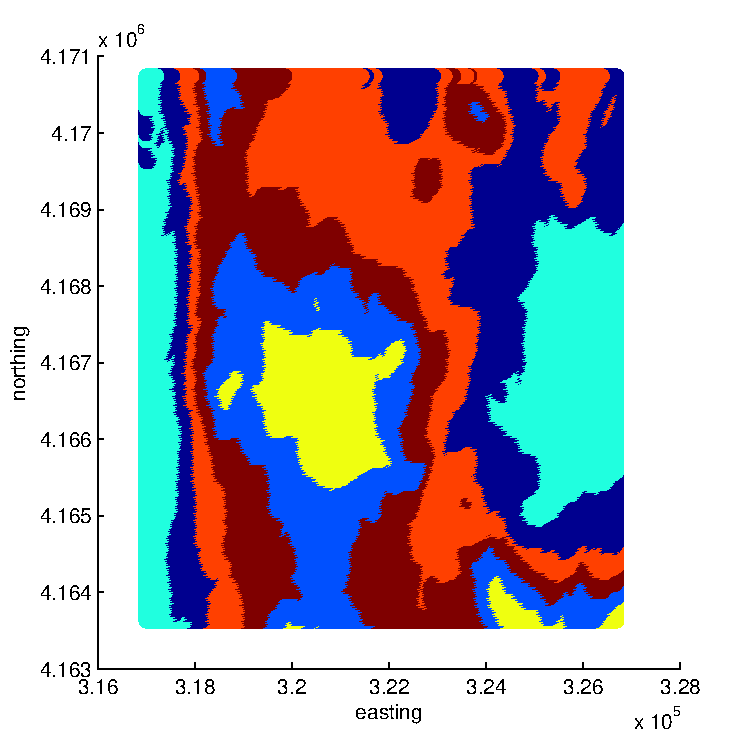
\includegraphics[width=8cm,height=7cm,keepaspectratio]{figs/Spectral_parallel.pdf}
 \caption{Parallel spectral clustering}
 \end{centering}
 \end{figure}

%\begin{figure}[H]
%  \begin{minipage}[b]{0.5\textwidth}
%    \begin{tabular}{c}
%      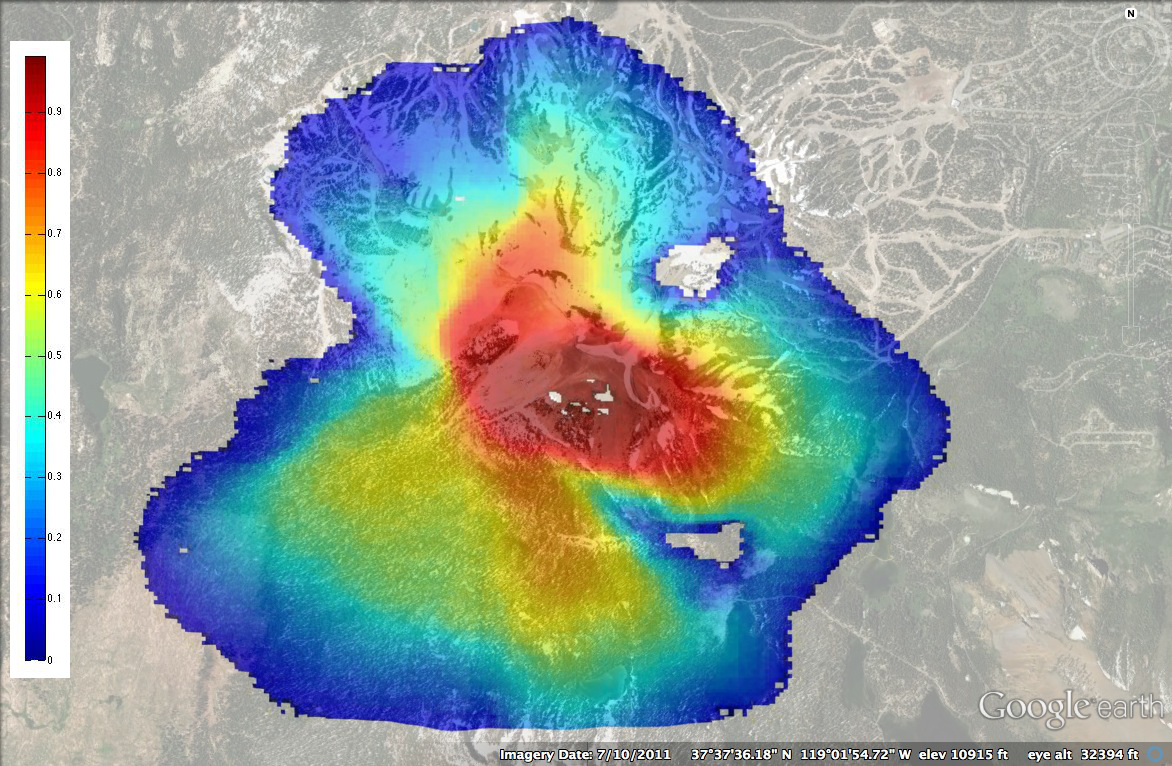
\includegraphics[width=8cm,height=7cm,keepaspectratio]{figs/hazard_map_noclusters.jpg}\\
%      (a)
%    \end{tabular}
%  \end{minipage}
%  % \hfill
%  \begin{minipage}{0.5\textwidth}
%    \begin{tabular}{c}
%      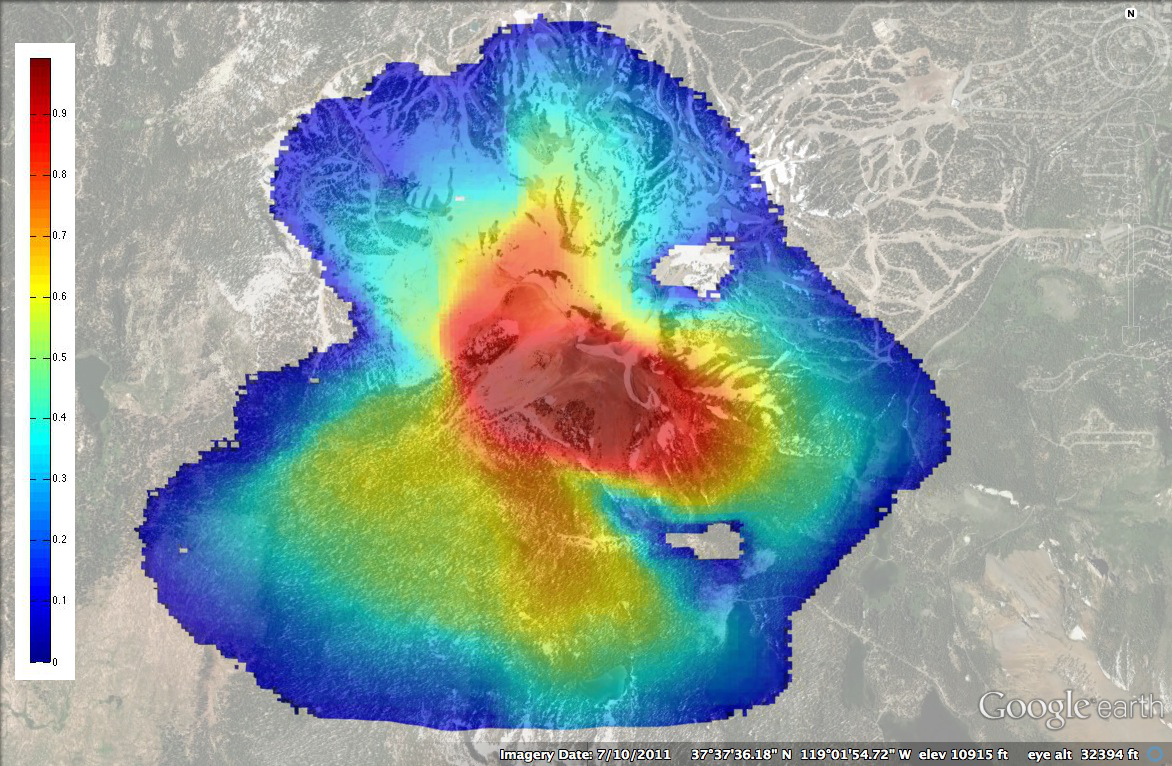
\includegraphics[width=8cm,height=7cm,keepaspectratio]{figs/hazard_map_clusters.jpg}\\
%      (b)
%    \end{tabular}
%  \end{minipage}
%  \caption{Hazard map a) no cluster b)clusters}\label{fig:fig5}
%\end{figure}


\section*{Acknowledgment}
 

\bibliographystyle{plainnat} \bibliography{mybib}
\end{document}